
\begin{frame}
  \frametitle{Un visualisateur de fichier DVI accéléré par GPU}
  \begin{center}
    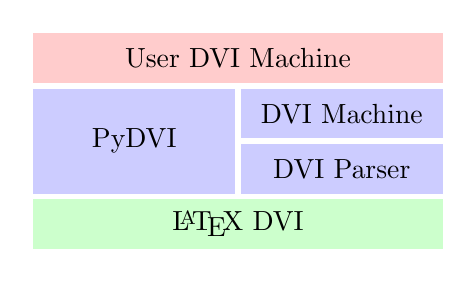
\begin{tikzpicture}[%
      base/.style={rectangle, minimum width=15em, minimum height=2em, draw=white, line width=2pt, anchor=south west},
      demibloc/.style={base, minimum width=7.5em}]
      \node[base, fill=green!20] at (0,0) {\LaTeX{} DVI};
      \node[demibloc, minimum height=4em, fill=blue!20] at (0,2em) {PyDVI};
      \node[demibloc, fill=blue!20] at (7.5em,2em) {DVI Parser};
      \node[demibloc, fill=blue!20] at (7.5em,4em) {DVI Machine};
      \node[base, fill=red!20] at (0,6em) {User DVI Machine};
    \end{tikzpicture}
  \end{center}
\end{frame}

%%% Local Variables: 
%%% mode: latex
%%% TeX-master: "master"
%%% End: 
